\section{Diseño}

Conforme a la metodología de desarrollo centrada en el usuario utilizada en este sistema, se decidió empezar por el desarrollo de un prototipo de alta fidelidad para el diseño del sistema, para posteriormente continuar con el diseño de la infraestructura y los sistemas necesarios para entregar el proyecto, con el objetivo de crear un sistema integral que pudiera satisfacer las necesidades del LCCA al mismo tiempo que cumpliera con los requisitos técnicos necesarios para cumplir los objetivos propuestos.

\subsection{Prototipado de la interfaz gráfica}

Para el desarrollo de un prototipo rápido de la interfaz gráfica, se utilizó el software \textit{Figma}, esto debido a que es un software gratuito, sencillo de utilizar orientado al prototipado de interfaces de alta fidelidad. \textit{Figma} ofrece la capacidad de integrar diferentes \textit{frameworks} de diseño de interfaces, para crear un \textit{design system} (un sistema de diseño) coherente, consistente a través de todo un proyecto. Utilizando este software se decidió utilizar una plantilla de un tablero de control para una plataforma genérica.

Los colores utilizados para el desarrollo de los prototipos, y posteriormente para el desarrollo de la totalidad del proyecto fueron; el color verde \texttt{\#09AB5D} como color principal de la interfaz, debido a su relación con el diseño actual del sitio de consulta de la información de las estaciones meteorológicas, y el color azul \texttt{\#16B2D4} como secundario por su contraste con el color verde y por su actual uso en el sitio existente del LCCA.

Utilizando esta plantilla como base para el lenguaje de diseño de la aplicación, se realizó un prototipado de la interfaz propuesta para evaluar la posible utilidad de la misma, creando un prototipo inicial de alta fidelidad. La primer interfaz en prototiparse fue el tablero de control, después de algunas iteraciones con cambios menores, el prototipo quedó tal como en la Figura \ref{fig:prototype_main_interface}, cabe notar que esta interfaz gráfica tiene elementos en la barra lateral que no corresponden con el proyecto (tal como la sección de chat y otros similares), esto debido a que se dejaron ciertos elementos predefinidos de la plantilla original, para no romper con la estética del diseño.

\begin{figure}[!ht]
	\centering
	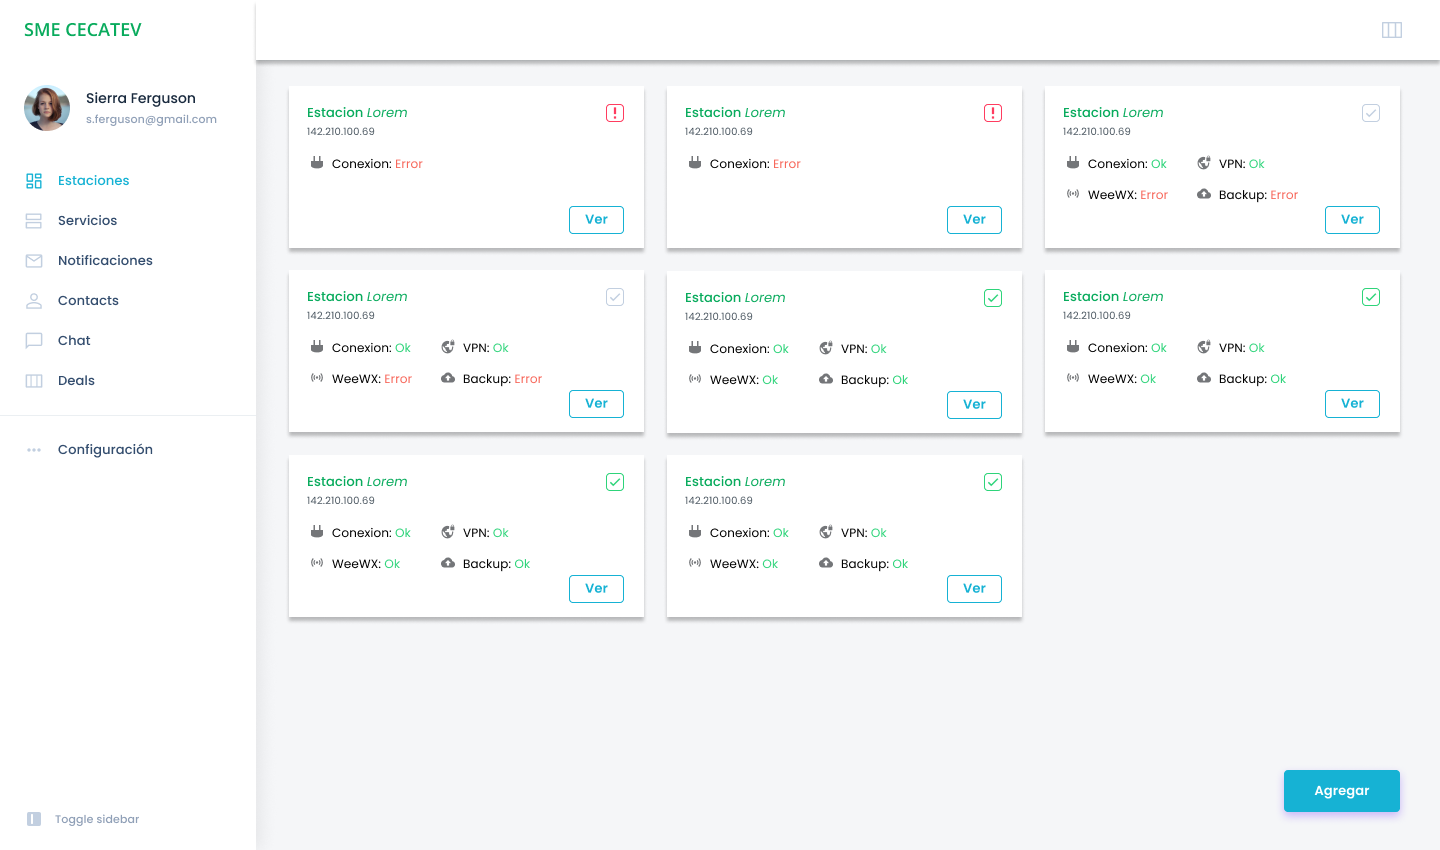
\includegraphics[width=1\linewidth]{images/diagrams/0.0.0_Main_interface.png}
	\caption{Prototipo del tablero de control.}
	\label{fig:prototype_main_interface}
\end{figure}

En este prototipo de interfaz se tomaron en cuenta en varios factores, uno de ellos, es que una estación que es monitoreada puede tener un error de conexión que no permita el acceso a la misma, y que al encontrarse con un error de conexión, no es posible obtener el estado de los servicios. De ser así, la información de estos servicios no se muestra. También se tomó en cuenta el identificar las estaciones por un nombre particular, pero también tener presente la dirección IP de la misma (en caso de poseer una) para volver más sencillo el acceso técnico a la información en caso de ser necesario para un usuario técnico. Además, se hizo la consideración de tener una variedad de diferentes servicios que se podrían monitorear, y que el estado de los servicios y de las estaciones fuera independiente.

\pagebreak

La segunda interfaz que fué elegida para su prototipado, fué la interfaz para agregar una nueva estación meteorológica al sistema. Esta interfaz contiene la información elemental que se requiere para registrar una nueva estación. En este caso, se compone de una dirección IP, un usuario, el método de conexión a la misma, el tipo de estación y el dispositivo por el que se accede a la misma. El prototipo realizado se puede observar en la Figura \ref{fig:prototype_add_station}

\begin{figure}[!ht]
	\centering
	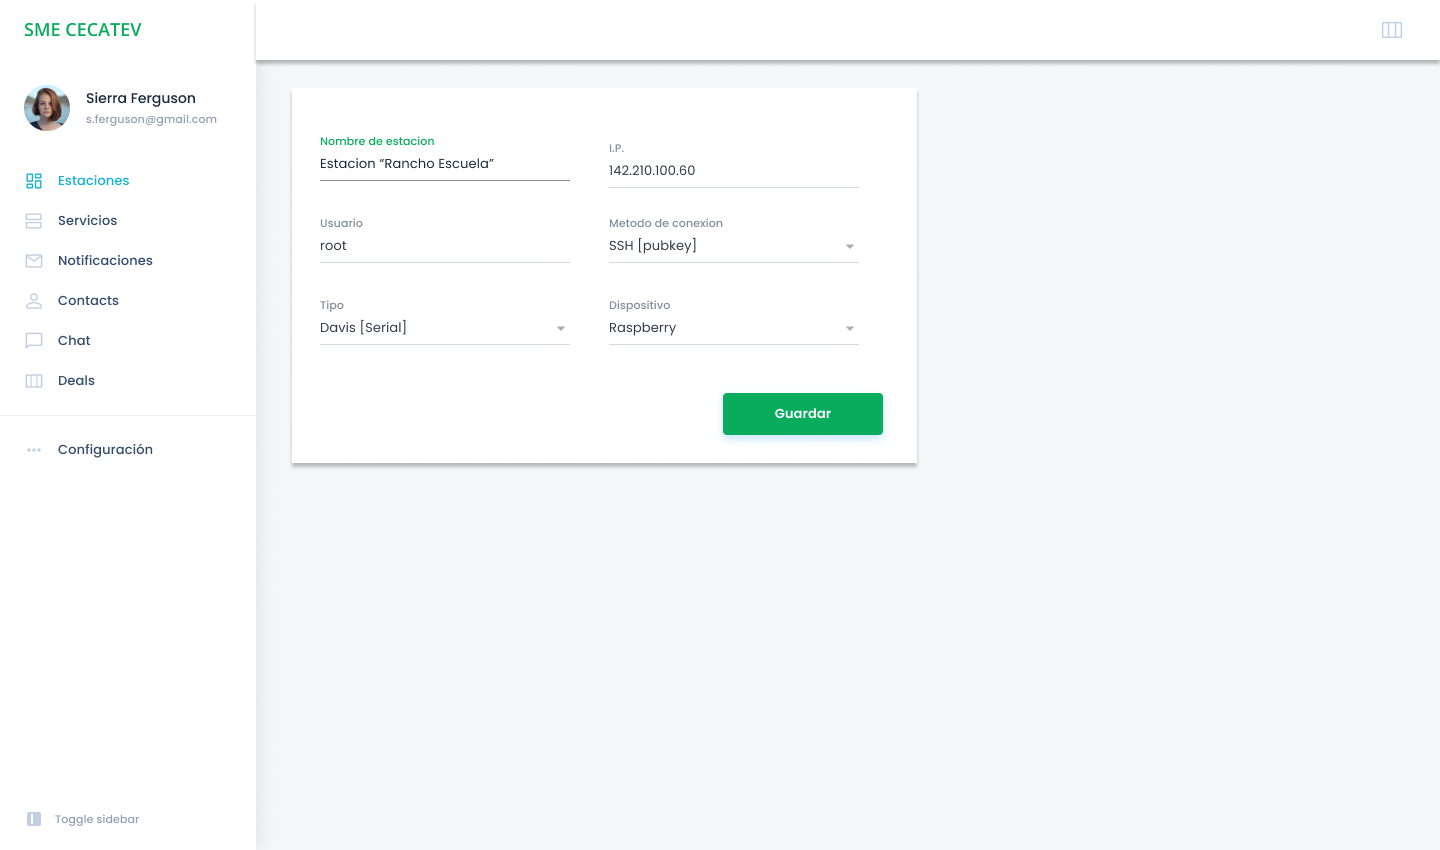
\includegraphics[width=1\linewidth]{images/diagrams/1.0.0_Stations_add.png}
	\caption{Prototipo de la interfaz para agregar una nueva estación.}
	\label{fig:prototype_add_station}
\end{figure}

\pagebreak

Posteriormente se creó el componente de la tercera parte importante del monitoreo de las estaciones meteoreológicas, el prototipo de la interfaz de solución de problemas de las estaciones. Al ser un objetivo secundario importante el poder tener y acceder a la información que las estaciones meteorológicas generan, se considera igualmente importante el poder capturar una razón de la solución de los inconvenientes para futuros análisis. Esta información será capturada con la ayuda de una interfaz como la de la Figura \ref{fig:prototype_solve_error}.

\begin{figure}[!ht]
	\centering
	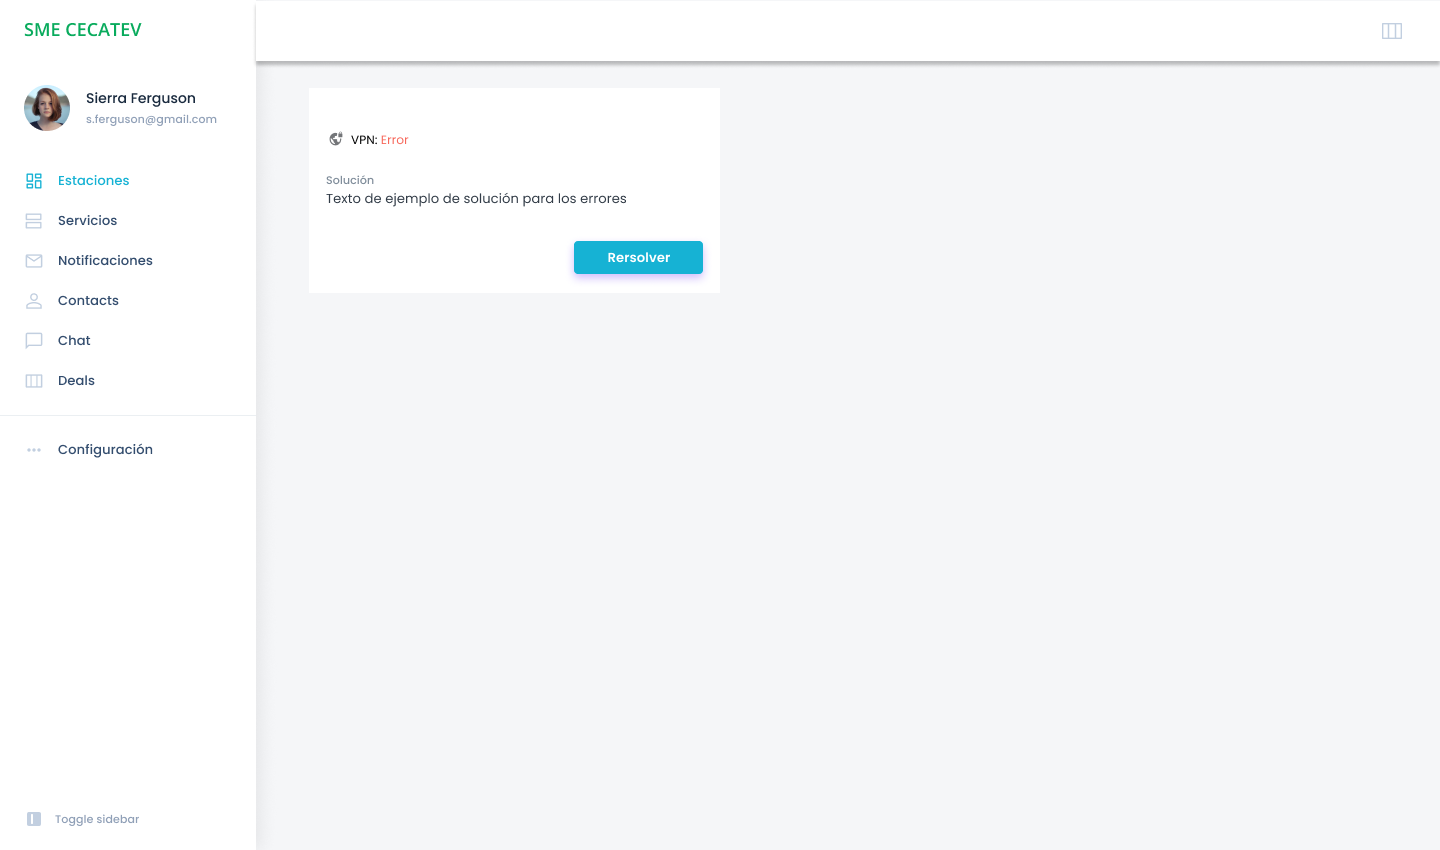
\includegraphics[width=1\linewidth]{images/diagrams/0.1.1_Station_Failing.png}
	\caption{Prototipo de la interfaz de solución de errores.}
	\label{fig:prototype_solve_error}
\end{figure}

\subsection{Diseño de base de datos}

Para el diseño de base de datos del sistema se consideraron dos elementos como relevantes, los datos de las estaciones meteorológicas, que incluyen datos como la conexión a las estaciones y la forma en la que se accederá a ellas, y los eventos que las mismas generen.

Si bien es posible almacenar la información de las estaciones meteorológicas en una \textit{time series database}, en la que la información del estado de cada uno de los servicios y elementos que se monitorean es almacenado sin importar el estado de los mismos, no se considera necesaria la información de los sistemas en su estado funcional, esto debido a que el volumen de datos generado, \textit{O(n*t*s)}, donde \textit{n} es el número de estaciones, \textit{t} la cantidad de veces que la inforamción se consulta por hora y \textit{s} el número de servicios que se consultan, es más grande que la utilidad que se le piensa dar a la información.

La información más relevante que se puede obtener de acuerdo a los objetivos de este proyecto es el estado de las estaciones de monitoreo en caso de falla, así como estimados de la calidad y accesibilidad de los datos que las estaciones recolectan.

Debido a esto, la base de datos se diseñó con el objetivo de almacenar la información en forma de eventos, y tomando en cuenta la utilidad futura de auditoría se decidieron agregar tiempos de creación de eventos y de la solución de los mismos. De la misma forma, el borrado de información no está contemplado en el sistema, para esto se implementó la metodología de borrado de información por medio de \textit{borrados suaves}, los cuales desactivan los registros lógicamente en el sistema sin borrar de forma física los datos de la base de datos.

En cuanto al manejo de la información adicional de las estaciones meteorológicas, es decir, la información de las mismas que no es indispensable para el funcionamiento del sistema pero es necesaria para controles internos, se agregó una tabla de atributos extra. Esta tabla contiene información diversas de las estaciones, y consiste en la forma \textit{llave -> valor} para los campos, esto, para asegurar la mayor flexibilidad posible de los datos y su almacenamiento. Sacrificando velocidades de indexamiento y procesamiento por una mayor libertad para extender y modificar el sistema.

Con todas estas consideraciones en mente, se creó una base de datos que corresponde con los contenidos que se muestran en el modelo entidad-relación que se puede obeservar en la Figura \ref{fig:diagrama_base_de_datos}.

% Agregar formas normales, y documentar mi proceso de normalización actual de las tablas.

\begin{figure}[!ht]
	\centering
	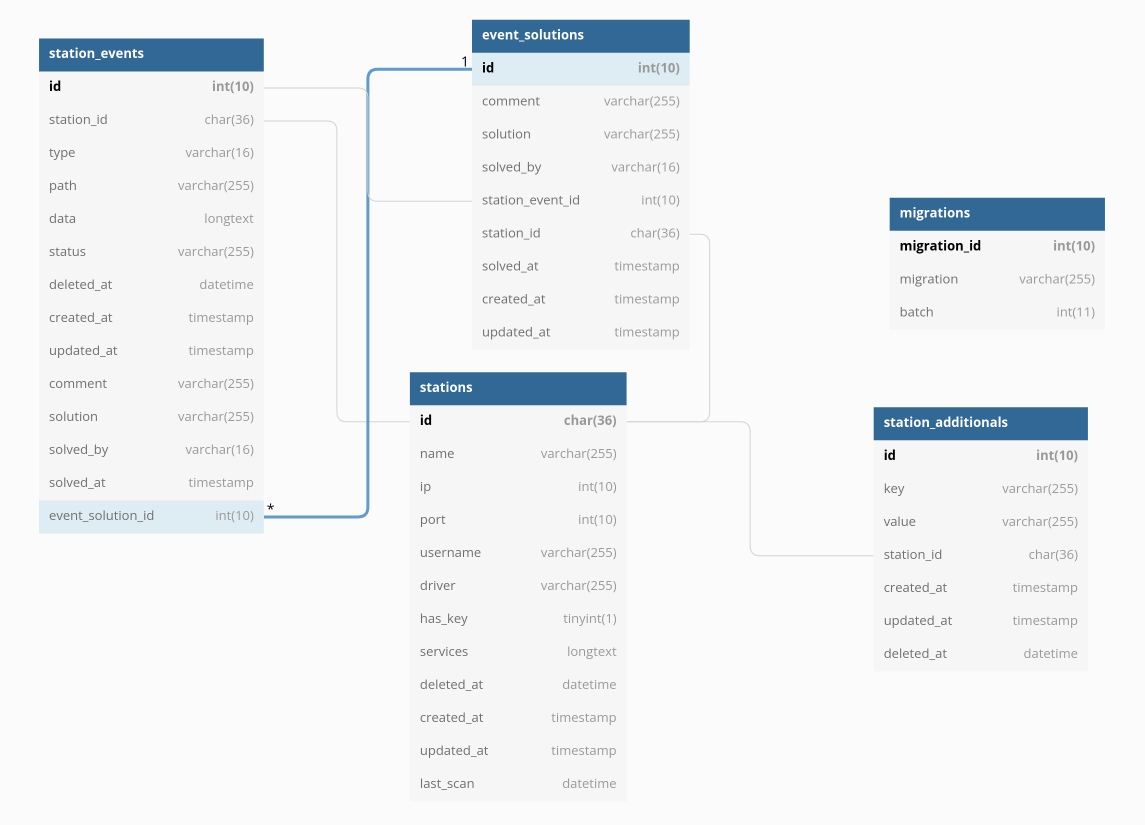
\includegraphics[width=0.86\linewidth]{images/diagrams/database_diagram.png}
	\caption{Modelo entidad-relación del proyecto meteoreo}
	\label{fig:diagrama_base_de_datos}
\end{figure}

\subsection{Arquitectura del sistema}

Para realizar la conexión a las estaciones meteorológicas, se decidió dividir el proyecto en dos componentes principales, un módulo de generación de reportes y un sistema de controladores que contuvieran el código de conexión y restauración de reportes de las estaciones.

Los drivers se desarrollaron con el objetivo de tener una plataforma estándar para la consulta de los datos de las estaciones.

Tomando como referencia el proyecto de \textit{Monitoring Plugins} \cite{monitoring_plugins}, el cual es compatible con diversos proyectos especializados en monitoreo de sistemas de alta resilencia, tales como \textit{Nagios} y \textit{Icinga}, se decidió crear un proyecto basado en drivers fácilmente extendibles.

%! TODO: Todo el desarrollo de la arquitectura del sistema

\subsection{Selección del motor de base de datos}

Para el caso de uso del centro de monitoreo de estaciones meteorológicas de la UACJ, en el que la red actual cuenta con 13 estaciones, no es necesario considerar como cuello de botella el motor de base de datos que se utilizará para el sistema. Esto debido a que, con un tiempo mínimo para la consulta del estado de las estaciones de hasta 5 minutos entre consultas, el sistema podría funcionar incluso con un tiempo promedio de 23 segundos desde la consulta hasta el almacenamiento de la información. Esto, sin tomar en cuenta que es posible paralelizar el proceso de consulta y generación de eventos de las estaciones meteorológicas, por lo que no se considera como algo relevante la selección de un motor de base de datos que cuente con alto rendimiento de lectura y/o escritura de la información.

Debido a que la infraestructura del sistema de las estaciones meteorológicas ya utiliza un motor relacional de base de datos adecuado para el proyecto, MySQL, se pretende utilizarlo para este proyecto, reduciendo la carga de mantenimiento para el equipo de la universidad, además de un sistema familiar que permitirá a los involucrados realizar consultas a la información sin necesidad de aprender nuevas tecnologías.

Para esto, se utilizó la flexibilidad que ofrecen los sistemas modelado de objetos y roles (ORM, por sus siglas en inglés) \cite{Halpin2006}, en la que se permite el crear sistemas agnósticos de un motor de base de datos en específico, y la creación de modelos, esquemas y relaciones de base de datos se dejan al \textit{framework} de modelado de datos. Esto además ofrece soporte para migraciones para realizar actualizaciones de base de datos controladas en caso de requerir extender un sistema existente.

El motor de base de datos seleccionado para el desarrollo local del proyecto fué el conocido como \textit{SQLite}, debido a la flexibilidad que ofrece al ser una base de datos que sólo depende de un archivo para funcionar y que no requiere de instalar paquetes de software extra en la estación que se utiliza para desarrollar y probar el proyecto.

\subsection{Configuración de ambiente de
desarrollo}\label{configuraciuxf3n-de-ambiente-de-desarrollo}

El ambiente de desarrollo que se seleccionó para la sección de python del proyecto fué seleccionado con el objetivo de proveer la mayor flexibilidad y portabilidad a corto y largo plazo, haciendo fácil la modificación posterior del proyecto por los que no estuvieron involucrados inicialmente, y sencillo de replicar para futuras investigaciones. Para lograr estos objetivos, se optó por realizar el proyecto con ayuda de las tecnologías de \textit{Docker}, debido a que permite realizar imágenes de proyectos de forma sencilla, y permite hacer contenedores multiplataforma que con una mínima configuración se vuelven útiles para el desarrollo.

% Con la finalidad de tener un contenedor de desarrollo que pueda ser replicado con la mínima configuración se eligió la plataforma docker, por su amplia adopción y por las facilidades que ofrece para crear sistemas complejos que dependen de varios servicios sin tener que realizar configuraciones en el sistema que puedan ser perdidas al momento de cambiar a otro.

Debido a la sencillez que el sistema de cnfiguración de contenedores \emph{docker compose} ofrece, se eligió para almacenar los parámetros de configuración de los contenedores en vez de crear comandos compatibles con docker para ello. Esto permite una fácil edición de los servicios y la aplicación de los mismos de una forma estandarizada que permite una comprensión más eficaz de los parámetros y de las dependencias.

El archivo de configuración fué almacenado en la raíz del proyecto, con el nombre de \texttt{docker-compose.yml}  tal como el estándar de la utilería \texttt{docker-compose} sugiere, y este archivo tiene el contenido siguiente que se muestra en el listado \ref{lst:docker-compose}. En este archivo, se especifica que se requiere de un servicio de \textit{MySQL}, el cuál fué utilizado para corroborar que el desarrollo era de utilidad con el motor seleccionado para producción, así como una referencia al archivo \textit{Docker} en el que se tiene el contenedor que se utilizará para el desarrollo. Además, se hace referencia a algunas variables, como \texttt{MYSQL\_DATABASE}, que son obtenidas de un archivo \texttt{\.env} estandarizado en la raíz del proyecto.

%! TODO: INSERTAR Referencia de archivo docker-compose en el anterior parrafito
% Cambiar líneas de configuracion por su relativo en texto y explicarlo en el párrafo
\begin{listing}
\begin{minted}{yaml}
version: '3.3'
services:
  api:
    container_name: meteoreo-api
    build:
      context: ./
      dockerfile: Dockerfile
    # ...
    # Configuración del ambiente
    # ...
    networks:
      - meteoreo-backend
  mysql:
    image: mysql
    container_name: meteoreo-mysql
    environment:
      MYSQL_DATABASE: '${MYSQL_DATABASE}'
      MYSQL_ROOT_PASSWORD: '${MYSQL_ROOT_PASSWORD}'
      MYSQL_PASSWORD: '${MYSQL_PASSWORD}'
      MYSQL_USER: '${MYSQL_USER}'
      SERVICE_TAGS: dev
      SERVICE_NAME: mysql
    ports:
      - '3306:3306'
    networks:
      - meteoreo-backend
networks:
  meteoreo-backend:
    driver: bridge
\end{minted}
\caption{Archivo docker-compose}
\label{lst:docker-compose}
\end{listing}

El archivo de \textit{docker-compose} tiene una dependencia con un archivo de Docker, que se pretende que facilite la adición de librerías adicionales al proyecto en la posteridad. Actualmente, extiende la imagen existente de \textit{tiangolo}, el proyecto \textit{Uvicorn-Gunicorn-Fastapi}. Esta imagen fue utilizada como base debido a su increíble flexibilidad para el desarrollo de proyectos en FastApi, sus optimizaciones automáticas para el balanceo de cargas entre diversos procesos creados automáticamente (ya que python es monoproceso) y además, por ser una imagen altamente mantenida por la comunidad, debido a su popularidad. En este archivo también se especifíca el instalar la librería \texttt{inteutils-ping} debido a que el proyecto dependerá de realizar pruebas por \texttt{ping} para revisar la conectividad con las estaciones antes de intentar realizar una conexión y la imagen base no tenía esta librería, el archivo final quedó como se muestra en el Listado \ref{lst:dockerfile}.

%! TODO: Insertar referencia de dockerfile en el anterior parrafito

\begin{listing}[h]
\begin{minted}{dockerfile}
FROM tiangolo/uvicorn-gunicorn-fastapi:python3.7

# Installs lib to do pings from the server
RUN apt-get update && apt-get install -y \
   inetutils-ping \
   && rm -rf /var/lib/apt/lists/*

CMD [ "/start-reload.sh" ]
\end{minted}
\caption[Dockerfile]{Archivo Dockerfile}
\label{lst:dockerfile}
\end{listing}

El editor de código seleccionado para el desarrollo del proyecto es Visual Studio Code, el cual posee una gran extensibilidad y predeterminados sensibles que permiten configurar el ambiente de trabajo de la forma que más sea conveniente para el desarrollo del proyecto, además provee la funcionalidad de \textit{devcontainers}, los cuales son parte de una extensión que permiten el crear ambientes de desarrollo dentro de ambientes virtuales en docker, utilizando las herramientas instaladas en la imagen de docker y que no requieren de configuración adicional por parte del desarrollador para comenzar a trabajar en un proyecto. Al detectar un archivo \texttt{devcontainer.json}, esta extensión automáticamente informa al desarrollador de su existencia y le invita a iniciar su ambiente de desarrollo utilizando los parámetros definidos en el arhivo.

En este archivo se especifica un nombre para identificar el ambiente de desarrollo que sea reconocible por el desarrollador, la localización del archivo que describe el contenedor, y una lista de extensiones para el editor de código. Entre las más importantes se encuentra \emph{pylance} que permite  realizar el formato automático de códgo con pep8 y \emph{magicpython} una adición al editor de código que provee un motor de autocompletación para python, las demás siendo preferencias personales útiles para agilizar el desarrollo del proyecto.

%! TODO: Insertar referencia del archivo devcontainer en el parrafito anterior

\begin{minted}{json}
{
  "name": "Meteoreo API",
  "service": "api",
  "remoteUser": "root",
  "shutdownAction": "stopCompose",
  "workspaceFolder": "/app",
  "dockerComposeFile": "../docker-compose.yml",
  "extensions": [
    "editorconfig.editorconfig",
    "mikestead.dotenv",
    "njpwerner.autodocstring",
    "aaron-bond.better-comments",
    "mhutchie.git-graph",
    "hookyqr.beautify",
    "magicstack.magicpython",
    "gruntfuggly.todo-tree",
    "ms-python.vscode-pylance",
    "sleistner.vscode-fileutils"
  ]
}
\end{minted}

Para el desarrollo de la sección de la interfaz de web del proyecto, se instaló en la máquina de desarrollo NPM versión 14.8.1, debido a que era la última versión \textit{LTS} (Soporte a largo plazo, por sus siglas en inglés) disponible, y el sistema de manejo de dependencias \textit{yarn} debido a las ventajas que ofrece sobre \textit{npm}, tales como mayor velocidad de instalación de paquetes y caché multiproyecto. No se vió como un elemento necesario el intergrar Docker o algún otro tipo de tecnología de contenedores para el proyecto de frontend, debido a la ubicuidad de las herramientas y la simpleza de instalación y de mantenimiento de las mismas.
